\clearpage
%//==============================--@--==============================//%
\subsection[3.5 Connection-Oriented Transport: TCP]{\hspace*{0.075 em}\raisebox{0.2 em}{$\pmb{\drsh}$} Connection-Oriented Transport: TCP}
\label{subsec:TCP}

%//==============================--@--==============================//%
\subsubsection[3.5.1 The TCP Connection]{$\pmb{\rightarrow}$ The TCP Connection}

\begin{itemize}
    \item \textbf{Connection-oriented:} TCP establishes a connection through a \underline{handshake} before data can be exchanged between application processes.
    
    \item \textbf{Logical connection:} The TCP connection is not an end-to-end circuit but a logical one, with common state residing only in the TCPs of the communicating end systems.
    
    \item \textbf{Full-duplex service}: TCP connections allow \underline{simultaneous data flow} in both directions between two processes.
    
    \item \textbf{Point-to-point:} TCP connections only involve a single sender and a single receiver, with \underline{multicasting not possible}.
    
    \item \textbf{Three-way handshake:} To establish a TCP connection, the client and server exchange three special TCP segments, setting up the parameters for the data transfer.
    
    \item \textbf{Send and receive buffers:} Each side of the connection has its own send buffer and its own receive buffer. The client process passes a stream of data through its socket, and TCP directs this data to the connection's send buffer. From time to time, TCP grabs chunks of data from the send buffer and passes it to the network layer.
    
    \item \textbf{Maximum Segment Size (MSS):} Maximum amount of application-layer data in a segment, typically determined by the \textbf{Maximum Transmission Unit (MTU)} for the local sending host. ``Ethernet and PPP link-layer protocols have an MTU of 1,500 bytes. Thus, a typical value of MSS is 1460 bytes.''\cite{Kurose2017}
    
    \item \textbf{TCP segments:} TCP pairs each chunk of client data with a TCP header, forming TCP segments, which are passed to the network layer and encapsulated within network-layer IP datagrams.
\end{itemize}

%//==============================--@--==============================//%
\subsubsection[3.5.2 TCP Segment Structure]{$\pmb{\rightarrow}$ TCP Segment Structure}

\vspace{-0.5em}
\begin{figure}[H]
    \centering
    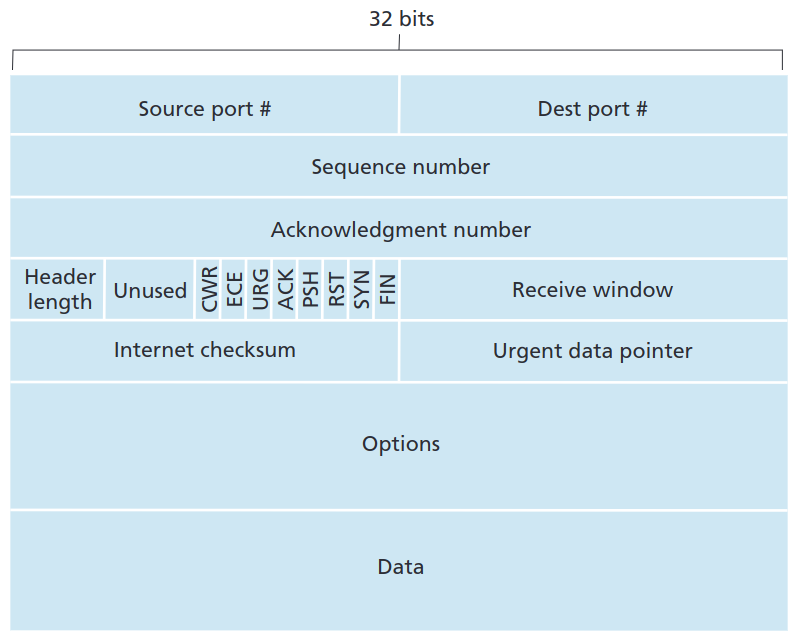
\includegraphics[width = 0.55\linewidth]{img/3/TCP-segment.png}
    \caption{Estrutura de um segmento TCP (consists of a header and payload). The header contains essential information, such as source and destination port numbers, sequence numbers, acknowledgment numbers, and flags. Additionally, the header includes the window size, checksum, and urgent pointer fields.}
    \label{fig:seg-TCP}
\end{figure}

\begin{itemize}
    \item \textbf{Sequence Numbers and Acknowledgment Numbers}
    \begin{itemize}
        \item Sequence numbers are over the stream of transmitted bytes, not over the series of transmitted segments.
        \item Acknowledgment numbers indicate the sequence number of the next byte the host is expecting.
        \item TCP provides \textbf{cumulative acknowledgments}, only acknowledging bytes up to the first missing byte in the stream.
        \item Initial sequence numbers are randomly chosen to minimize possible confusion with segments from earlier connections.
    \end{itemize}
    
    \item \textbf{Header Fields}
    \begin{itemize}
        \item \textbf{Source and destination port numbers}: for multiplexing/demultiplexing data from/to upper-layer applications.
        \item \textbf{Checksum field}
        \item 32-bit \textbf{sequence number field} and 32-bit \textbf{acknowledgment number field}: used for reliable data transfer service
        \item 16-bit \textbf{receive window field}: used for flow control, indicating the number of bytes that a receiver is willing to accept
        \item 4-bit \textbf{header length field}: specifies the length of the TCP header in 32-bit words
        \item \textbf{Optional} and \textbf{variable-length options field}: used for negotiating the MSS, window scaling factor, and time-stamping option
        \item \textbf{Flag field}: contains 6 bits (ACK, RST, SYN, FIN, CWR, and ECE) for various purposes
        \item \textbf{Urgent data pointer}: indicates the location of the last byte of urgent data
    \end{itemize}
\end{itemize}

%//==============================--@--==============================//%
\subsubsection[3.5.3 Round-Trip Time Estimation and Timeout]{$\pmb{\rightarrow}$ Round-Trip Time Estimation and Timeout}

\begin{mdframed}
    \vspace{-1.15 em}
    \begin{align*}
        \texttt{EstimatedRTT} &= \texttt{EstimatedRTT} \cdot (1 - \alpha) + \texttt{SampleRTT} \cdot \alpha \\
        \texttt{DeviationRTT} &= \texttt{DeviationRTT} \cdot (1 - \beta) + \left\vert\, \texttt{SampleRTT} - \texttt{EstimatedRTT}\, \right\vert \cdot \beta \\[-6pt] \cline{1-2}
        \texttt{Timeout} &= \texttt{EstimatedRTT} + 4 \cdot \texttt{DeviationRTT}
    \end{align*}
\end{mdframed}

\noindent \textbf{Nota:} Valores típicos para: $\alpha = 0.125 = 1/8$ $[$RFC 6298$]$, $\beta = 0.25 = 1/4$.

\renewcommand*{\thefootnote}{\fnsymbol{footnote}}
\footnotetext[4]{%
    ``Note that \texttt{EstimatedRTT} is a weighted average of the \texttt{SampleRTT} values. (...) this weighted average puts more weight on recent samples than on old samples. This is natural, as the more recent samples better reflect the current congestion in the network. In statistics, such an average is called an \textbf{exponential weighted moving average (EWMA)}.''\cite{Kurose2017}
}
\renewcommand*{\thefootnote}{\arabic{footnote}}

%//==============================--@--==============================//%
\subsubsection[3.5.4 Reliable Data Transfer]{$\pmb{\rightarrow}$ Reliable Data Transfer}
 
 Com base no discutido na \hyperref[subsec:reliable-data-transfer]{secção \textbf{Reliable Data Transfer}}, o protocolo utilizado pelo TCP é o \textbf{temporizador/janela e ACKs cumulativos}, possuindo também uma forma rudimentar de controlo de congestão que passa pela duplicação dos intervalos de \textit{timeout}: ``(...) each time TCP retransmits, it sets the next timeout interval to twice the previous value $[$sofre um crescimento exponencial$]$ (...) However, whenever the timer is started after data is received from the application above or an ACK is received, the \texttt{TimeoutInterval} is derived from the most recent values of \texttt{EstimatedRTT} and \texttt{DeviationRTT}."\cite{Kurose2017}

%//==============================--@--==============================//%
\subsubsection[3.5.5 TCP Flow Control]{$\rightarrow$ TCP Flow Control}

TCP flow control prevents sender-induced buffer overflow at the receiver, ensuring efficient data transmission. It uses a sliding window mechanism to adjust the transmission rate according to the receiver's buffer capacity and network conditions.

\vspace{-0.5em}
\begin{enumerate}
    \item \textbf{Receiver buffer and advertised window (\texttt{rwnd})}: The receiver allocates a buffer, with spare room defined as:
          \begin{equation*}
            \texttt{rwnd} = \texttt{RcvBuffer} - [\texttt{LastByteRcvd} - \texttt{LastByteRead}]
          \end{equation*}
          The sender is informed of \texttt{rwnd} via the Window field in TCP headers.
          
    \item \textbf{Sliding window and flow control operation}: The sender adjusts its sending window based on \texttt{rwnd} and network conditions. It stops transmitting data if \texttt{rwnd} drops to zero and resumes when a non-zero \texttt{rwnd} value is received.
    
    \item \textbf{Handling zero \texttt{rwnd}}: If \texttt{rwnd} is zero and the receiver has no data or ACKs to send, the sender continues sending one-byte segments to keep the receiver updated about its buffer state.
    
    \item \textbf{Interaction with congestion control}: Flow control works with congestion control mechanisms like slow start and congestion avoidance to adapt the transmission rate to both the receiver's buffer capacity and network bandwidth.
\end{enumerate}

%//==============================--@--==============================//%
\subsubsection[3.5.6 TCP Connection Management]{$\rightarrow$ TCP Connection Management}

The connection management process is mainly driven by a three-way handshake and a four-way handshake for connection establishment and termination, respectively.

\vspace{-0.5em}
\begin{enumerate}
    \item \textbf{Three-way handshake (Connection Establishment)}: The handshake process involves three steps:
        \begin{enumerate} \small
            \item SYN: The client sends a TCP segment with the SYN (synchronize) flag set, indicating a connection request.
            \item SYN + ACK: The server responds with a segment with both the SYN and ACK (acknowledge) flags set, acknowledging the client's request and synchronizing its own sequence number.
            \item ACK: The client sends an ACK segment, confirming the establishment of the connection.
        \end{enumerate}
    \item \textbf{Data transmission}: Once the connection is established, data transmission occurs using the sliding window and congestion control mechanisms.
    \item \textbf{Four-way handshake (Connection Termination)}: The termination process involves the following steps:
        \begin{enumerate} \small
            \item FIN: The endpoint initiating the connection termination sends a segment with the FIN (finish) flag set, signaling the desire to close the connection.
            \item ACK: The other endpoint acknowledges the FIN segment with an ACK segment.
            \item FIN: The other endpoint also sends a FIN segment to indicate it is ready to close the connection.
            \item ACK: The initiating endpoint acknowledges the second FIN segment with an ACK segment, completing the termination process.
        \end{enumerate}
\end{enumerate}

\renewcommand*{\thefootnote}{\fnsymbol{footnote}}
\footnotetext[4]{%
    \textbf{TCP Connection States}: During connection management, both client and server transition through various states such as LISTEN, SYN-SENT, SYN-RECEIVED, ESTABLISHED, FIN-WAIT-1, FIN-WAIT-2, CLOSING, TIME-WAIT, CLOSE-WAIT, LAST-ACK, and CLOSED.
}
\renewcommand*{\thefootnote}{\arabic{footnote}}
%//==============================--@--==============================//